\documentclass[../Interim_Report_Master]{subfiles}
\begin{document}
\hypertarget{drop_mod}{\section{Droplet Evaporation Model}\label{drop_mod}}
\subsection{Definition of Models} 
The 8 models in \cite{Miller1998} are denoted by Mx where x is the model number.

What defines the models are the variables \(f_{1}\), \(f_{2}\), \(Nu\), \(Sh\) \(H_{\Delta T}\) and \(H_{M}\). Although the main variation in the models stems from \(f_{2}\), \(H_{\Delta T}\) and \(H_{M}\). M1 is known as the classical rapid mixing model. M2 will be ruled out for the purposes of this project as the $B'_T$ term in the evaporation correction $f_2$ must be solved iteratively at each timestep. This increases the computation overhead of the simulation which may be acceptable for a single droplet but will be problematic for large population of droplets.
\begin{table}[h]
	\centering
	\begin{tabular*}{\textwidth}{c @{\extracolsep{\fill}} cccc}
		\hline
		\textbf{Model} & \textbf{Name} & \textbf{$f_2$} & \textbf{$H_{\Delta T}$} & \textbf{$H_M$} \\ \hline
		\textbf{M1} & Classical rapid mixing & $1$ & $0$ & $\ln \left[1+B_{M,eq}\right]$ \\[2ex] 
		\textbf{M2} & Abrmazon-Sirignano & $\frac{-\dot{m}_{d}}{{m}_{d}B'_{T}}\left[\frac{3Pr_{G}\tau_{d}}{Nu}\right]$ & $0$ & $\ln \left[1+B_{M,eq}\right]$ \\[2ex] 
		\textbf{M3} & Mass analogy Ia & $1$ & 0 & $B_{m,eq}$ \\[2ex]
		\textbf{M7} & Langmuir-Knudsen I & $\frac{\beta}{e^{\beta}-1}$ & $\frac{2\beta}{3Pr_G}\left(\frac{\theta_1}{\tau_d}\right)\Delta_s$ & $\ln \left[1+B_{M,neq}\right]$ \\[2ex] \hline
	\end{tabular*}
	\caption{Detail of variables used in candidate models.}
\end{table}

A more suitable model to provide a point of comparison in this case would be one of the mass analogy models, M3-M6. Which are derived from vapour mass fraction boundary condition at the droplet's surface. This assumes the droplet does not dissolve in the gas phase. These models use the same formulations for the surface vapour mass fraction ($Y_s$), Spalding transfer number for mass ($B_m$) and mass transfer potential ($H_{\Delta T}$). This would simplify producing code for an extra model.

Models M7 and M8, are to be ruled out as they use non-equilibrium formulations of the coefficients which would further complicate the code. The comparison between models is left as future work. With the choice of model for this project will be M1 due to its wide usage and ease of implementation

\subsection{Assumptions}
The model presented here is subject to the following assumptions:
\begin{enumerate}
	\item The droplets are formed of a single species
	\item The droplet is spherical and remains spherical for the entire evaporation process
	\item There is no interaction between droplets
	\item Within the droplet there is 
		\begin{enumerate}
			\item Zero temperature gradient
			\item Zero concentration gradient
		\end{enumerate}
	\item The droplet temperature is homogeneous
	\item The properties of the carrier gas are constant and are unaffected by the process of droplets evaporating
\end{enumerate}

\cite{Miller1998}\cite{arnold2000}.

\subsection{Governing Equations}
Each of the models are defined by the same four Lagrangian equations for the droplets:
\begin{align}
\frac{dX_{i}}{dt} &= v_{i} 
\label{vel} \\
\frac{dv_{i}}{dt} &= \left(\frac{f_{1}}{\tau_{d}}\right)(u_{i}-v_{i}) + g_i 
\label{accel} \\
\frac{dT_{d}}{dt} &= \frac{f_{2}Nu}{3Pr_{G}}\left(\frac{\theta_1}{\tau_d}\right)(T_{G}-T_{d}) + \left(\frac{L_{V}}{C_{L}}\right)\frac{\dot{m}_{d}}{m_{d}} - H_{\Delta T} 
\label{temp} \\
\frac{dm_{d}}{dt} &= -\frac{Sh}{3Sc_{G}}\left(\frac{m_{d}}{\tau_{d}}\right)H_M
\label{mass}
\end{align}

\subsubsection{Particle Timescales}
$\tau_d$ is the momentum relaxation timescale for the particle. This provides a timescale for each particle. It is determined from:
\begin{equation}
\tau_d = \frac{\rho_d D^2}{18\mu_G}
\end{equation}

There is an equivalent timescale for the heat transfer process. This can be derived from equation \ref{heat_sol_an} as:
\begin{equation}
\tau_T = \tau_d\left(\frac{3Pr_G}{Nu f_2 \theta_1}\right)
\end{equation}
%\begin{equation}
%%\tau_T = \frac{\rho_d C_{p,G}D^2}{12\lambda_l}
%\tau_T = \frac{\rho_d C_{p,L}D^2}{12\lambda_G}
%\end{equation}

%Similarly for the mass transfer:
%\begin{equation}
%\tau_m = \tau_d\left(\frac{3Sc_G}{Sh}\right)
%\end{equation}

These two timescales are exceptionally useful for the non-dimensionalisation of results. This provides a way of evaluating how quickly processes occur in the timescale of the particle. Which is a far more useful insight into the physics taking place than particle x takes y seconds to evaporate.

\subsubsection{Position}
Equation \ref{vel} and a simpler form of equation \ref{accel} were used in the IP this project is based off. The differential equation for position was solved using the trapezoidal rule, as this method has second order accuracy and the result is a linear first order equation:
\begin{equation}
X_{n+1} = X_{n} + \frac{v_{n}+v_{n+1}}{2} \Delta t
\end{equation}

\cite{Elijah_GPU_Report}

\subsubsection{Velocity}
For equation \ref{accel}, the acceleration of the droplet is defined using Stokes' Law and can be derived by considering the forces acting on the particle:
\begin{figure}
	\centering
	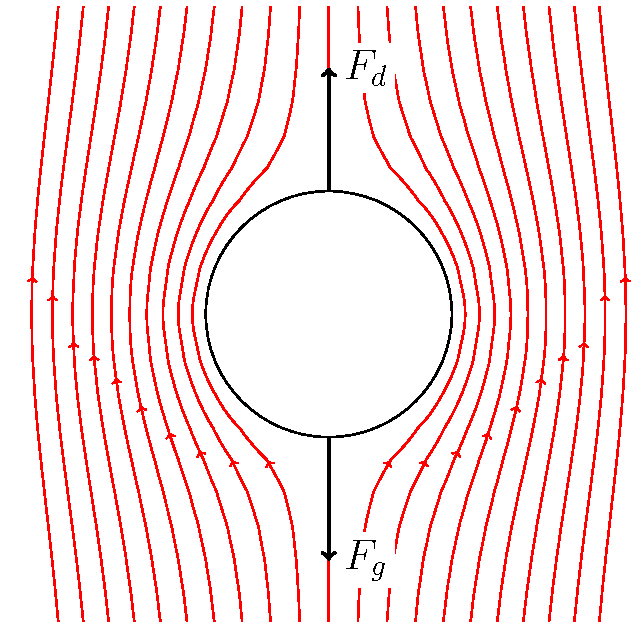
\includegraphics[width=0.5\textwidth]{./Diagrams/Particle_Forces/Particle_Forces.pdf}
	\caption{Forces acting on a particle under a Stokes flow regime.}
	\label{particle_forces}
\end{figure}

The total force acting on the particle is:
\begin{equation}
F = F_g + F_d
\end{equation}

This can be solved as a differential equation:
\begin{subequations}
	\begin{align}
	F &= ma \\
	F &= m\frac{du}{dt} \\
	\frac{du}{dt} &= \frac{F(u)}{m}
	\end{align}
\end{subequations}

The force acting on the particle is the sum of the weight and drag forces. The weight force is given by:
\begin{equation}
F_g = mg
\end{equation}

It is assumed the particle experiences a Stokes drag regime, therefore:
\begin{equation}
F_d = \frac{m}{\tau_d}(u_f-u)
\end{equation}

So, the differential equation is:
\begin{subequations}
	\begin{align}
	\frac{du}{dt} &= \frac{F(u)}{m} \\
	\frac{du}{dt} &= \frac{F_g + F_d}{m} \\
	\frac{du}{dt} &= \frac{mg + \frac{m}{\tau_d}(u-v)}{m} \\
	\frac{du}{dt} &= \frac{1}{\tau_d}(u-v) + g
	\end{align}
\end{subequations}

This is for one vector component, hence the 3D case is:
\begin{equation}
\frac{dv_i}{dt} = \frac{1}{\tau_d}(u_i-v_i) + g_i
\end{equation}

is dependent on three terms. Acceleration due to gravity \(g_{i}\), and the difference between the carrier gas velocity and the velocity of the particle, \(u_{i}-v_{i}\). The third term is a correction for Stokes drag that is dependent on the time constant for Stokes flow. 

A formulation for $f_1$ is given in \cite{Miller1998} as:
\begin{equation}
f_{1} = \frac{1+0.0545Re_{d}+0.1Re_{d}^{0.5}(1-0.03Re_{d})}{1+a|Re_{b}|^{b}}
\end{equation}

With the Reynolds numbers defined as:
\begin{subequations}
\begin{align}
Re_d &= \frac{\rho_G u_s D}{\mu_G} \\
Re_b &= \frac{\rho_G u_b D}{\mu_G} 
\intertext{The velocities defined as:}
u_s &= |u_i-v_i| \\
u_b &= -\frac{\dot{m}}{\pi \rho_G D^2 u_b}
\intertext{And the constants $a$ and $b$ defined as:}
a &= 0.09 + 0.077\exp(-0.4Re_d) \\
b &= 0.4 + 0.77\exp(-0.04Re_d)
\end{align}
\end{subequations}

Which is an empirical result produced from a data fit. In this format it is valid for $0\leq Re_d \leq 100$ and $0\leq Re_b \leq 10$. For the purpose of this research $f_1$ will be set to $1$. This reduces the computation per timestep and still allows for comparisons to be made with data in the literature. As the models can be driven by iterating from an initial Reynolds number instead of using equation \ref{accel}.

\subsubsection{Temperature}
The temperature ODE is a combination of a convective and diffusive processes. The convection is determined by:
\begin{equation}
\dot{Q} = \frac{Nu}{\tau_d}(T_G-T_d)
\end{equation}

\subsubsection{Mass}

 
\end{document}